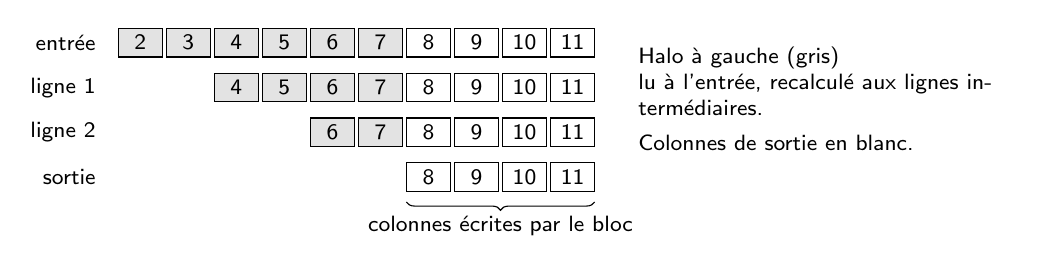
\begin{tikzpicture}[x=.61cm,y=.57cm,font=\footnotesize\sffamily,inner sep=1pt]
\foreach \r/\start/\nom in {0/2/entrée,1/4/ligne 1,2/6/ligne 2,3/8/sortie} {
  \node[anchor=east] at (1.14,-\r) {\nom};
  \foreach \c in {\start,...,11} {
    \ifnum\c<8\relax
      \draw[fill=black!11] (\c-.46,-\r-.32) rectangle (\c+.46,-\r+.32);
    \else
      \draw[fill=white] (\c-.46,-\r-.32) rectangle (\c+.46,-\r+.32);
    \fi
    \node at (\c,-\r) {\c};
  }
}
\draw[decorate,decoration={brace,mirror,amplitude=3pt}] (7.54,-3.55)--(11.46,-3.55)
  node[midway,below=4pt] {colonnes écrites par le bloc};
\node[anchor=west,align=left,text width=50mm] at (12.3,-1.25)
  {Halo à gauche (gris)\par lu à l’entrée, recalculé aux lignes intermédiaires.\par
   \smallskip Colonnes de sortie en blanc.};
\end{tikzpicture}
